\subsection{Identifying Component 3 in Figure T-3}
\label{T6C10}

\begin{tcolorbox}[colback=gray!10!white,colframe=black!75!black,title=T6C10]
What is component 3 in figure T-3?

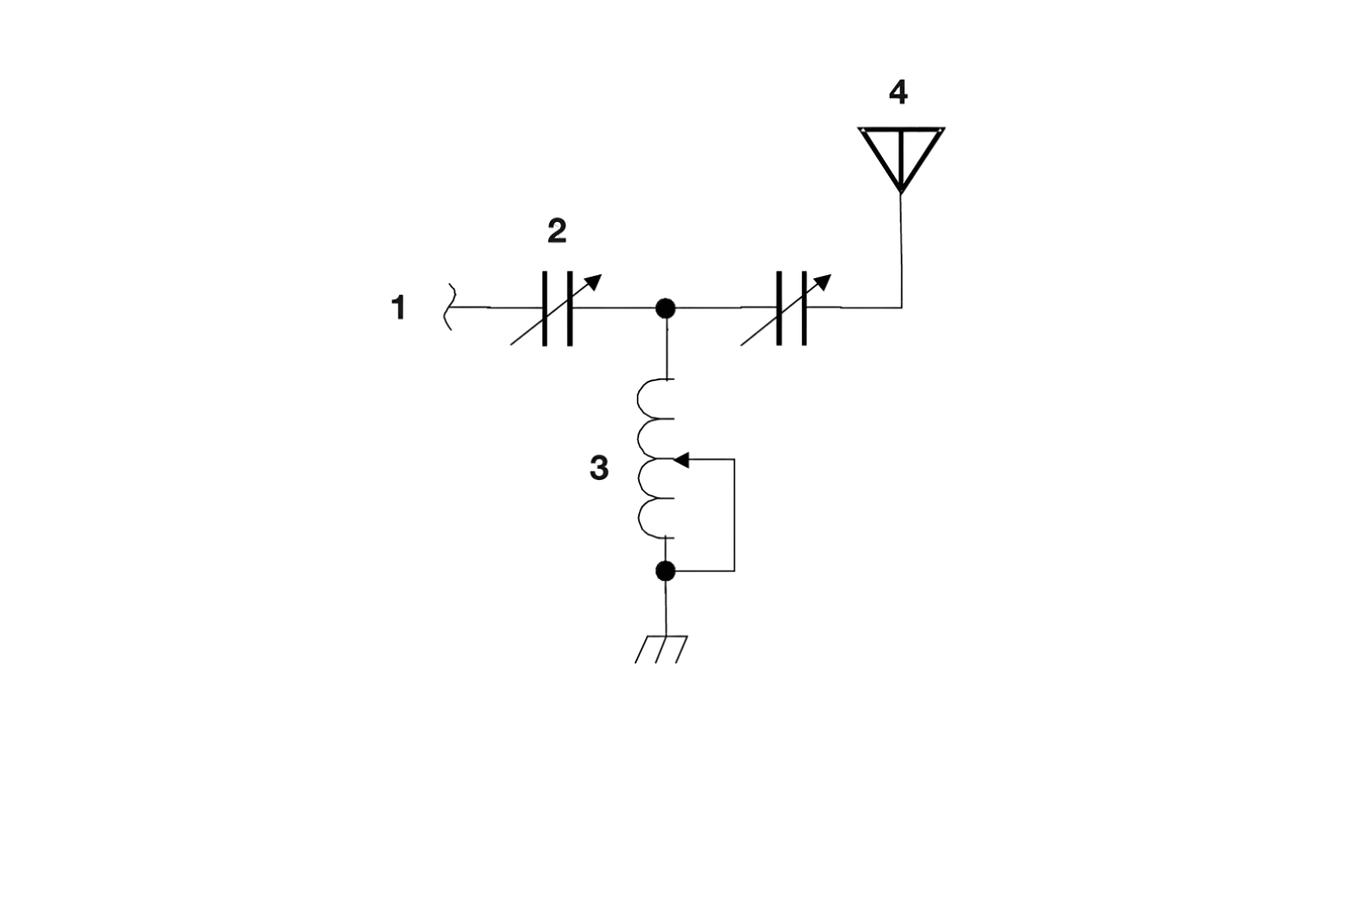
\includegraphics[width=0.5\textwidth]{tech/images/t3.png} 

\begin{enumerate}[label=\Alph*)]
    \item Connector
    \item Meter
    \item Variable capacitor
    \item \textbf{Variable inductor}
\end{enumerate}
\end{tcolorbox}

\subsubsection{Intuitive Explanation}
Imagine you have a magic wand that can change how much it resists the flow of electricity. Now, in figure T-3, component 3 is like that magic wand, but instead of resisting, it changes how much it holds back the electricity in a special way. It's not a connector, a meter, or a variable capacitor—it's a variable inductor! Think of it as a coil that can adjust how much it spins the electricity around.

\subsubsection{Advanced Explanation}
In the context of radio technology, a variable inductor is a component that allows the inductance to be adjusted. Inductance, denoted by \( L \), is a property of an electrical conductor by which a change in current induces an electromotive force (EMF) in both the conductor itself and in any nearby conductors. The unit of inductance is the henry (H).

A variable inductor typically consists of a coil of wire with a movable core. By adjusting the position of the core, the inductance can be varied. This is particularly useful in tuning circuits, where precise control over the inductance is required to match the resonant frequency of the circuit.

Mathematically, the inductance \( L \) of a coil can be approximated by:
\[ L = \frac{\mu N^2 A}{l} \]
where:
\begin{itemize}
    \item \( \mu \) is the permeability of the core material,
    \item \( N \) is the number of turns in the coil,
    \item \( A \) is the cross-sectional area of the coil,
    \item \( l \) is the length of the coil.
\end{itemize}

By changing the position of the core, the effective permeability \( \mu \) changes, thereby altering the inductance \( L \).

% Prompt for generating the diagram: 
% A diagram showing a variable inductor with a movable core, labeled as component 3 in figure T-3. The diagram should illustrate how the core's position affects the inductance.